\chapter{Auswertung}

Nach erfolgreichem Abschluss des Reihungstests, kann die Auswertung gestartet werden. Klicken Sie hierzu auf der Administratorseite rechts oben auf 'Auswertung'.\\
\\
Hier kann der entsprechende Reihungstest und Studiengang ausgew�hlt und die Auswertung erstellt werden.\\

\begin{figure}
	\centering
	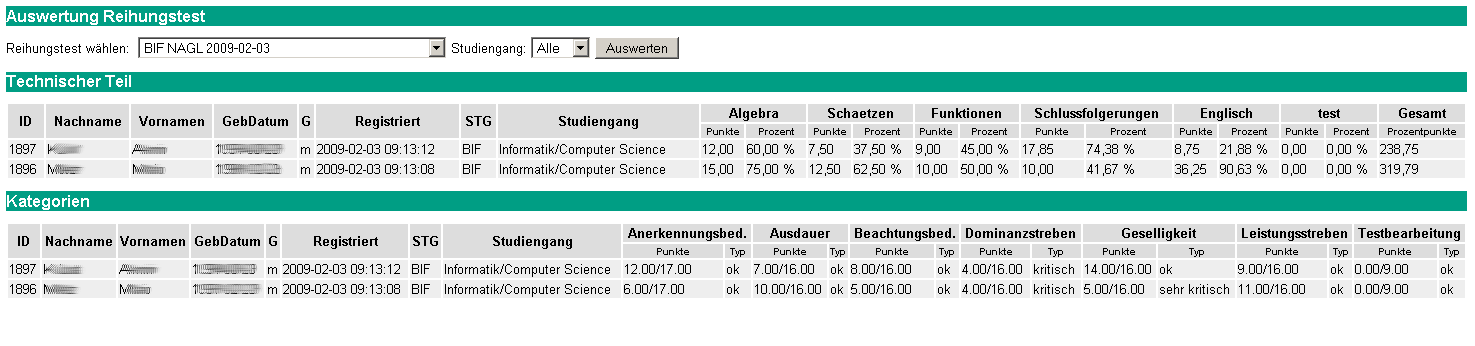
\includegraphics[width=0.75\textwidth]{testtool_auswertung.png}
	\caption{Auswertung des Reihungstests}
	\label{Auswertung des Reihungstests}
\end{figure}
\section{�bernehmen der Punkte ins FAS-Online}

Es gibt mehrere M�glichkeiten die Reihungstestpunkte ins FAS-Online zur �bernehmen:\\
\\
\begin{itemize}
\item Punkte einer einzelnen Person direkt im FAS abfragen
\item Punkte aller Personen eines Reihungstests ins FAS �bertragen
\item Punkte einer einzelnen Person aus der Reihungstestverwaltung �bertragen
\end{itemize}

\subsection{Punkte einer einzelnen Person direkt im FAS abfragen}

Im FAS k�nnen �ber den Karteireiter Prestudent, die Reihungstestpunkte einer einzelnen Person �bertragen werden. Klicken sie hierzu auf das Symbol neben dem Punkt Punkte1 im Abschnitt Reihungstest um die Punkte zu holen.

\begin{figure}
	\begin{center}
    \begin{picture}(100,51)
			\put(20,0){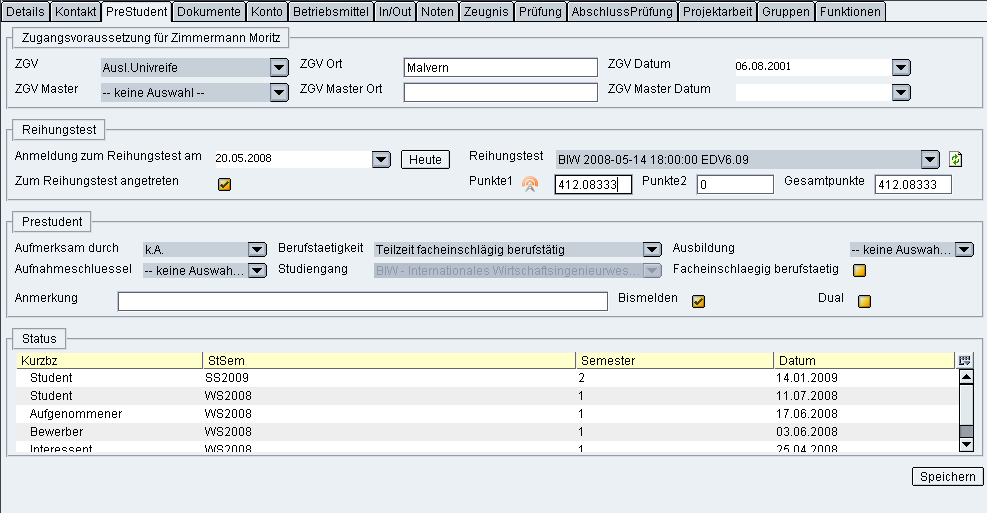
\includegraphics[height=51mm, width=100mm]{FAS_Prestudent1.png}}
			\markier{1}{68}{38}{1}{-1}
		\end{picture}
    \caption{�bertragen der Punkte}
		\label{�bertragen der Punkte}
  \end{center}
\end{figure}

Sie m�ssen anschlie�end auf Speichern dr�cken damit die Punkte gespeichert werden.\\
\\
\\
\\

\subsection {Punkte aller Personen eines Reihungstests ins FAS �bertragen}

�ber den Men�punkt Extras->Reihungstestverwaltung im FAS gelangen Sie zur �bersichtsseite �ber die vorhandenen Reihungstests. Wenn Sie einen Reihungstest ausw�hlen der bereits abgeschlossen ist, erhalten sie die M�glichkeit �ber den Link 'alle Punkte ins FAS �bertragen' die Punkte aller Personen dieses Reihungstests ins FAS zu �bertragen.

\begin{figure}
	\begin{center}
    \begin{picture}(100,51)
			\put(20,0){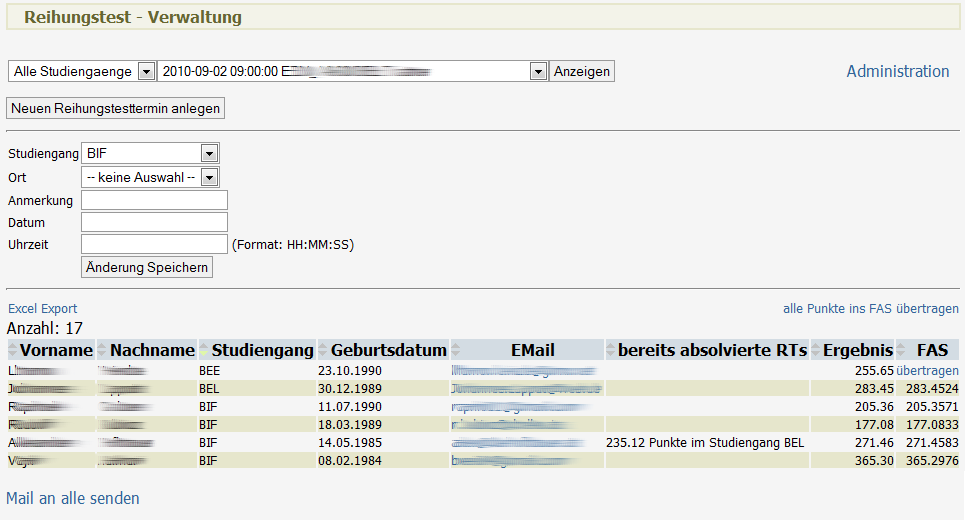
\includegraphics[height=51mm, width=100mm]{FAS_Reihungstest1.png}}
			\markier{1}{97}{27}{1}{-1}
		\end{picture}
    \caption{�bertragen der Punkte}
		\label{�bertragen der Punkte}
  \end{center}
\end{figure}

\subsection{Punkte einer einzelnen Person aus der Reihungstestverwaltung �bertragen}

�ber die Reihungstestverwaltung k�nnen Sie auch die Punkte einzelner Personen ins FAS �bertragen wenn Sie auf den Link '�bertragen' klicken.
